\documentclass{article}
\usepackage{amsmath}
\usepackage{amssymb}
\usepackage{graphicx}
\begin{document}
	\section[Parallel]{Simple Parallel (Tank Circuit) Resonance }
	When the inductor and capacitor have equal reactances, the circuit is in a 
	state of resonance.  The frequency at which this occurs is known as the 
	resonant frequency and is given by:
	$$ 2 \pi f L = \frac{1}{2 \pi f C}$$ 
	$$ f^2 = \frac{1}{4\pi ^2 C L}$$
	\begin{equation}\label{eq:res-freq}
	f_{\text{res}}=\frac{1}{2\pi \sqrt{LC}}
	\end{equation}
	\subsection[ZeroR]{Zero Resistance}
	Assuming the resistance is zero, a simple LC parallel circuit will have an 
	undefined impedance -- more specifically, the reciprocal of zero, which is 
	a domain error/undefined -- and a current of zero at resonance.  This is 
	due to the notion that at resonance, the two components will have equal 
	reactances but opposing phase shifts, or, in other words, the complex 
	number representations of their impedance wave forms will have equal 
	magnitude but opposite directions.
	$$ Z_T = \frac{1}{\frac{1}{Z_L} + \frac{1}{Z_C}}$$
	Let '$D$' be defined as:
	$$ D := \frac{1}{Z_L} + \frac{1}{Z_C} = \frac{1}{X_L}\angle-90^{\circ} + 
	\frac{1}{X_C}\angle90^{\circ} = j \cdot \left(\frac{1}{X_C} - \frac{1}{X_L} 
	\right) = 
	0$$
	Thus:
	$$ Z_T = \frac{1}{D} = \frac{1}{0} = \text{undefined}$$
	The amplitude of the current is given by:
	$$ |I|(f \vert L, C, E_T) = \frac{E_T}{|Z_T|}$$
	$$ |Z_T| = \frac{1}{|D|} $$
	$$ \frac{1}{|Z_T|} = \left| \frac{1}{X_C} - \frac{1}{X_L}\right | = \left| 
	2\pi f C - 
	\frac{1}{2 \pi f L} \right |$$
	$$ \frac{1}{|Z_T|} = \left | \frac{V_\theta^2 CL - 1}{V_\theta L} \right|$$
	\subsection[NonZeroR]{Non-zero Resistance}
	Realistically, except in the case of a superconductor, there will be some 
	resistance.  Assuming this resistance is in parallel with the LC parallel 
	circuit, at resonance, the impedance will have a magnitude that is 
	equal to the this resistance with a phase shift of zero.
	\paragraph[In Parallel]{When in parallel} with the tank circuit, the total 
	impedance is given by:
	$$ Z_T = \frac{1}{D + \frac{1}{Z_R}} = Z_R = R\angle0$$
	And the amplitude of the current:
	$$ |I|(f\vert R, L, C, E_T) = \frac{|E_T|}{|Z_T|}$$
	Let '$D$' be redefined as:
	$$ D := \frac{1}{X_R} + j \cdot \left( \frac{1}{X_C} - 
	\frac{1}{X_L}\right)$$
	It then follows that,
	$$|D| = \left|j \cdot \left( \frac{1}{X_C} - \frac{1}{X_L}\right) + 
	\frac{1}{X_R}\right|=\sqrt{\frac{1}{R^2} + \left( \frac{1}{X_C} - 
	\frac{1}{X_L} \right)^2}$$
	And that:
	$$ |Z_T| = \frac{1}{|D|}$$
	Which means that:
	$$ |I| = |E_T| \cdot |D|$$
	\paragraph[In Series]{When in series} with the tank circuit, the total 
	impedance is given by:
	$$ Z_T = Z_R + \frac{1}{D} = X_R  + j \cdot  \frac{V_\theta L}{V_\theta^2 
	CL -1}$$
	And the amplitude of the current:
	$$ |Z_T| = \sqrt{R^2 + \frac{V_\theta^2L^2}{(V_\theta^2CL - 1)^2}}$$
	$$ |I|(f \vert R, L, C, E_T) = \frac{E_T}{|Z_T|}$$
	\section[Series]{Simple Resonance Series}
	When a capacitor and an inductor are connected in series to an AC power 
	supply, the magnitude of the impedance is equal to zero at resonant 
	frequency, assuming a resistance of zero.  This implies that the current 
	has an amplitude that is undefined, or, more specifically, an amplitude 
	that is equal to the magnitude of the supplied voltage, presumably a finite 
	positive value, divided by zero.
	$$ E_T = Z_T I$$
	$$ Z_T = Z_L + Z_C = j \cdot (X_L - X_C)$$
	Via the above equation, in conjunction with the fact that $X_C=X_L$, which 
	is implied by the assumption that we are at resonant frequency,
	$$ Z_T = 0$$
	Thankfully, for our safety, with the exception of superconductors, the 
	connecting wires typically have some resistance.  So even when there is no 
	resistor in the circuit, the magnitude of the impedance is not really equal 
	to zero and the amplitude of the current has a finite value.
	$$  Z_T = Z_R + Z_L + Z_C = X_R + j\cdot (X_L - X_C)$$
	At resonance, the total impedance is equal to the impedance derived from 
	the total resistance of the circuit. \\ \\
	As for the magnitude of the current:
	\begin{equation}\label{eq:simple-series-magZ_T}
		|Z_T| = \sqrt{R^2 + (X_L-X_C)^2}
	\end{equation}
	$$ |I| = \frac{|E_T|}{|Z_T|}$$
	\paragraph[Example 1]{For an example,} let '$|I|(f)$' be defined as:
	$$ |I|(f):=|I|(f \vert 1\Omega, 100\text{mH}, 10\mu\text{F}, 1\text{V})$$
	The resonant frequency of the circuit that fits these parameters is:
	$$ f_{\text{res}} = \frac{1}{2\pi \sqrt{0.1 \cdot 10^{-5}}} = \frac{10^3}{2 
	\pi }\approxeq 159.155 \text{Hz}$$
	And part of the curve given by $|I|(f)$ is found in figure 
	(\ref{fig:simple-series}).
	\begin{figure}[h]
		\label{fig:simple-series}
		\centering
		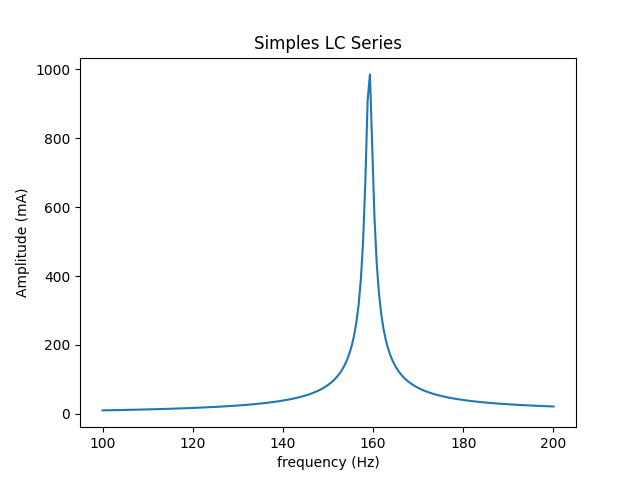
\includegraphics[width=0.784\linewidth,height=0.588\linewidth]{simple-series}
		\caption{Part of the curve given by |I|(f).}
	\end{figure}
	Notice how the amplitude peaks at the resonant frequency, which is 
	consistent with and imples that the total impedance is at it's minimum at  
	this frequency.  This is consistent with equation 
	(\ref{eq:simple-series-magZ_T}).
	\subsection[CriticalPnts]{Finding the Critical Points}
	The magnitude of the current is never zero -- it is always positive -- so 
	$|I|$ has no roots.  To find the critical points, denoted as '$P$', of the 
	curve given by this 
	function we must find the roots of the derivative, $|I|'(f)$. \\ \\
	Let $|I|(f)$ be redefined as:
	$$ |I|(f):=|I|(f \vert, R, L, C, E_T)$$
	$$ |I|'(f)=-|E_T|\frac{(X_L-X_C)\left(2\pi L + \frac{1}{2\pi 
	Cf^2}\right)}{\sqrt{\big(R^2+(X_L-X_C)^2\big)^3}} $$
	$$ |I|'(P_x)=0$$
	Multiplying throughout by the denominator and dividing throughout by the 
	constant factor gives:
	$$ (X_L(P_x) - X_C(P_x))\left(2\pi L + \frac{1}{2\pi C P_x^2}\right)=0$$
	To find the first pair of roots, divide throughout by the left factor.
	$$ 2\pi L + \frac{1}{2\pi C P_x^2} = 0$$
	$$ \frac{1}{2\pi C P_x^2} = - 2\pi L$$
	$$ P_x^2 = - \frac{1}{4\pi^2 C L}$$
	$$ P_x \supset \pm j \frac{1}{2\pi \sqrt{LC}} = \pm j \cdot f_{\text{res}} 
	$$
	Imaginary roots are not what we are looking for. \\ \\
	Now divide throughout by the right hand factor.
	$$ X_L(P_x) = X_C(P_x)$$
	$$ P_x^2 = \frac{1}{4\pi^2LC}$$
	$$ P_x \supset \pm \frac{1}{2 \pi \sqrt{LC}} = \pm f_{\text{res}} $$
	\section[Series-Parallel]{Resonance in Series-Parallel Circuits}
	Recall that the resonant frequency is given by:
	\begin{equation}\tag{\ref{eq:res-freq}}
		f_{\text{res}}=\frac{1}{2\pi \sqrt{LC}}
	\end{equation}
	The impedance of a parallel circuit with resonant frequency is equal to 
	infinity (assuming there is zero resistance, which only happens in a super 
	conductor), which implies that the current is equal to zero.  Conversely, 
	the impedance is equal to zero -- again, assuming zero resistance -- under 
	the same conditions in a simple series circuit, implying that the current 
	is of infinite magnitude or 
	amplitude.
	\subsection[High-Res]{Calculating the Resonant Frequency of a 
	High-Resistance Circuit}
	Suppose there is a circuit with an AC power supply of 
	$e:=E_T=1\text{V}\angle0$, a capacitor with a capacitance of 
	$C=10\mu\text{F}=10^{-5}\text{F}$ in parallel with a resistor with a 
	resistance of $R=100\Omega$ and an inductor with an inductance of 
	$L=100\text{mH}=0.1\text{H}$.  This supposed circuit is of the form 
	$C//(R--L)$.\\ \\
	The reactance of each component is given by:
	\begin{align*}
		X_C &= \frac{1}{2\pi f C} \\
		X_R &= R \\
		X_L &= 2\pi f L
	\end{align*}
	And the impedance:
	\begin{align*}
		Z_C &= X_C \angle-90^{\circ} \\
		Z_R &= X_R \angle 0 \\
		Z_L &= X_L \angle 90^{\circ}
	\end{align*}
	The total impedance is given by:
	\begin{equation}\label{eq:total-imp}
		Z_T = \frac{1}{\frac{1}{Z_C}+\frac{1}{Z_R+Z_L}}
	\end{equation}
	Via Ohm's Law,
	$$ E_T = Z_TI$$
	If we want to find the total current, denoted as '$I$', as a function of 
	the frequency, denoted as '$f$', then we need to multiply throughout by the 
	denominator of $Z_T$ in equation (\ref{eq:total-imp}).
	$$ I = E_T\left(\frac{1}{Z_C} + \frac{1}{Z_R+Z_L}\right)$$
	Let $Z_{R--L}:=Z_R + Z_L=R + j \cdot 2\pi f L$.  In polar form:
	$$ Z_{R--L} = \sqrt{R^2 + 4(\pi f L)^2}\angle \arctan \frac{2 \pi f L}{R}$$
	The reciprocal of the above:
	$$ \frac{1}{Z_{R--L}}=\frac{1}{\sqrt{R^2 + 4(\pi f L)^2}}\angle-\arctan 
	\frac{2 \pi f L}{R}$$
	In rectangular form:
	\begin{align*}
		\frac{1}{Z_{R--L}} &= 
		\frac{1}{|Z_{R--L}|}\left(\frac{R}{|Z_{R--L}|} - j\cdot\frac{2\pi f 
		L}{|Z_{R--L}|}\right) \\
		 &= \frac{R-j\cdot 2\pi f L}{R^2 + 4(\pi f L)^2}
	\end{align*}
	And, for the other term of the denominator of $Z_T$:
	$$ \frac{1}{Z_C} = 2\pi f C \angle 90^{\circ}$$
	In rectangular form:
	$$ \frac{1}{Z_C} = j \cdot 2\pi f C$$
	So the denominator is given by:
	\begin{align*}
		\frac{1}{Z_C} + \frac{1}{Z_R + Z_L} &= \frac{R}{R^2+4(\pi f L)^2} + j 
		\cdot 2 \pi f\left(C - \frac{L}{R^2+4(\pi f L)^2}  \right) \\
		 &= \frac{R + j \cdot 2\pi f \Big(C\big(R^2+4(\pi f L)^2\big) - 
		 L\Big)}{R^2+4(\pi f L)^2}
	\end{align*}
	And so the magnitude of the current as a function of the frequency is given 
	by:
	$$ |I|(f) = E_T \frac{\sqrt{R^2 + 4(\pi f)^2\Big(C\big(R^2+4(\pi f 
	L)^2\big) - L\Big)^2}}{R^2+4(\pi f L)^2}$$
	Now let '$V_\theta$' and '$W_\theta$' be defined as:
	$$ V_\theta:=V_\theta(f):=2\pi f$$
	$$ W_\theta:=W_\theta(f):=V_\theta^2$$
	Also note that the reactances of the capacitor and the inductor are a 
	function of the frequency.
	$$ X_C = X_C(f) = \frac{1}{V_\theta (f)C}$$
	$$ X_L = X_L(f) = V_\theta (f)L$$ 
	It then follows that $|I|(f)$ can be more concisely written as:
	$$ |I|(f) = E_T \frac{\sqrt{R^2 + W_\theta\big(C(R^2 +X_L^2 ) - 
	L\big)^2}}{R^2 + X_L^2}$$
	The amplitude at resonant frequency is:
	$$ |I|(f_{\text{res}}=159.159 \text{Hz}) \approx 7.071 \text{mA}$$
	To find the maximum amplitude of $I$ and the frequency at which it occurs, 
	we may need to find the root(s) of the derivative of $|I|(f)$.
	Let '$N$' and '$D$' be defined as:
	$$ N:=\sqrt{R^2 + 4(\pi f)^2\Big(C\big(R^2+4(\pi f 
		L)^2\big) - L\Big)^2}$$
	$$ D:=R^2+4(\pi f L)^2$$
	\begin{align*}
		|I|'(f) =&\frac {4\pi^2 E_T f}{N\cdot D} \Bigg(\Big(C\big(R^2+4(\pi f 
		L)^2\big) - L\Big)^2 +  2C(2\pi Lf)^2\Big(C\big(R^2+4(\pi f 
		L)^2\big) - L\Big)\Bigg) \\
		 -& \hspace{1ex}E_T \frac{8\pi^2L^2 f N}{D^2}
	\end{align*}
	Before even finishing the job of completely finding the derivative, it 
	appears that finding the roots would require finding the roots of a degree 
	six polynomial.  This will require some numerical method.
	\paragraph[Swap]{Now suppose the resistor} is on the other branch of the 
	parallel circuit.  Our supposed circuit now has the form: $(C--R)//L$.  The 
	amplitude of the current as a function of the 
	frequency is given by:
	$$ |I|(f) = E_T\left| \frac{1}{Z_C+Z_R} + \frac{1}{Z_L} \right|$$
	$$ \frac{1}{Z_L} = \frac{1}{2\pi f L}\angle-90^{\circ} = - j\cdot 
	\frac{1}{2\pi f L}$$
	$$ \frac{1}{Z_C + Z_R} = \frac{1}{X_R - j \cdot X_C} =  
	\frac{1}{\sqrt{X_R^2 + X_C^2}}\angle-\arctan -\frac{X_C}{X_R}$$
	Let '$Z_1$' be defined as: $Z_1:=Z_C+Z_R$.
	$$ \frac{1}{Z_1} = \frac{1}{|Z_1|} \left( \frac{X_R}{|Z_1|} + j 
	\frac{X_C}{|Z_1|}\right) = \frac{X_R + j \cdot X_C}{X_R^2 + X_C^2}$$
	$$ \frac{1}{Z_1} + \frac{1}{Z_L} = \frac{X_R}{|Z_1|^2} + j \left( 
	\frac{X_C}{|Z_1|^2} - \frac{1}{X_L}\right)$$
	$$ \left| \frac{1}{Z_1} + \frac{1}{Z_L} \right| = \sqrt{\frac{R^2}{|Z_1|^4} 
	+ \left(\frac{X_C}{|Z_1|^2} - \frac{1}{X_L}\right)^2}$$
	\subsection[LC Series]{Series LC Circuits}
	Suppose we have a circuit of the form: $\text{R1}$--C--L//$\text{R2}$.  
	The values of $C$ 
	and $L$ are the same as the previous subsection, while $R_1=1\Omega$ and 
	$R_2=100\Omega$.  To find the amplitude of the current as a function of the 
	frequency we first need to look at the total impedance of our circuit.
	\begin{equation}\label{eq:total-imp_2}
		Z_T = Z_{R1} + Z_C + \frac{1}{\frac{1}{Z_L} + \frac{1}{Z_{R2}}}
	\end{equation}
	To make the above equation more concise, let N0:=R1, N1:=C, N2:=L//R2, 
	N2A:=L, and N2B:=R2.  The impedance of each component follows the same 
	labeling/denoting scheme.  I.e. $Z0=Z_{R1}$ denotes the impedance of N0 or 
	R1 and $Z2A=Z_L$ denotes the impedance of N2A or L.  Thus we have a more 
	concise equation:
	\begin{equation}\tag{\ref{eq:total-imp_2}}
		Z_T = Z0 + Z1 + Z2
	\end{equation} 
	Note that '$Z2$' denotes the impedance of the parallel combination that is 
	in series with the rest of the circuit.
	$$ Z2 = \frac{1}{\frac{1}{Z2A} + \frac{1}{Z2B}}$$
	Recall from the previous subsection that:
	$$ \frac{1}{Z_L} = \frac{1}{V_\theta L}\angle-90^{\circ} = - j \cdot 
	\frac{1}{V_\theta L} = - j \cdot \frac{1}{X_L}$$
	$$ \frac{1}{Z_{R2}} = \frac{1}{R_2}\angle0 = \frac{1}{R_2}$$
	Adding them gives:
	$$ \frac{1}{Z2A} + \frac{1}{Z2B} = \frac{1}{R_2} - j \cdot \frac{1}{X_L}$$
	Let $D_{Z2}$ be defined as:
	$$ D_{Z2} := \frac{1}{Z2A} + \frac{1}{Z2B}= \frac{1}{R_2} - j \cdot 
	\frac{1}{X_L}$$
	The polar form is given by:
	$$ D_{Z2} = |D_{Z2}|\angle\arctan - \frac{R_2}{X_L}$$
	$$ |D_{Z2}| = \sqrt{\frac{1}{R_2^2} + \frac{1}{X_L^2}}$$
	It then follows that:
	$$ Z2 = \frac{1}{D_{Z2}} = \frac{1}{|D_{Z2}|}\angle-\arctan - 
	\frac{R_2}{X_L}$$
	To add the above impedance value with the impedance values of the 
	components that it's corresponding component is in series with, we need to 
	convert it into rectangular form.
	$$ Z2 = \frac{1}{|D_{Z2}|}\left( \frac{1}{R_2 |D_{Z2}|} + j \cdot 
	\frac{1}{X_L |D_{Z2}|} \right)$$
	And of course, $Z1$ in rectangular form is:
	$$ Z1 = - j \cdot X_C$$
	$$ Z_T = R_1 + \frac{1}{R_2|D_{Z2}|^2} + j \cdot \left( 
	\frac{1}{X_L|D_{Z2}|^2} - X_C \right)$$
	The magnitude of the total impedance is given by:
	\begin{equation}\label{eq:mag-total-imp_2}
		|Z_T| = \sqrt{\left( R_1 + \frac{1}{R_2|D_{Z2}|^2} \right)^2 + \left( 
		\frac{1}{X_L|D_{Z2}|^2} - X_C \right)^2}
	\end{equation}
	The amplitude of the current as a function of frequency is thus given by:
	$$ |I|(f) = \frac{E_T}{|Z_T|}$$
	\paragraph[Swap]{Now suppose } the inductor and capacitor swap places.  Our 
	supposed circuit now has the form of: R1--C//R2--L=R1--L--C//R2.  Note that 
	the category of circuit components, (CC, --, //), is commutative, hence the 
	equality of the two circuit expressions, both of which describe the 
	supposed circuit.  \\ \\
	The total impedance is:
	$$ Z_T=Z0+Z1+Z2$$
	$$ Z0=R_1\angle0=R_1$$
	$$ Z1=Z_L=X_L\angle90^{\circ}=j \cdot X_L$$
	Let $D_{Z2}$ be defined as:
	$$ D_{Z2} := \frac{1}{Z_{R2}} + \frac{1}{Z_C} = \frac{1}{R_2}\angle0 + 
	V_\theta C \angle 90^{\circ}$$
	And in rectangular form:
	$$ D_{Z2}=\frac{1}{R_2} + j \cdot V_\theta C$$
	In polar form:
	$$ D_{Z2}=|D_{Z2}|\angle\arctan (V_\theta C \cdot R_2)$$
	$$ |D_{Z2}| = \sqrt{\frac{1}{R_2^2} + W_\theta C^2}$$
	Finally, for our third term:
	$$ Z2 = \frac{1}{D_{Z2}}= \frac{1}{|D_{Z2}|}\angle - \arctan (V_\theta C 
	\cdot R_2)$$
	In rectangular form:
	$$ Z2 = \frac{1}{|D_{Z2}|}\left( \frac{1}{|D_{Z2}| \cdot R_2} - j \cdot 
	\frac{V_\theta C}{|D_{Z2}|} \right)$$
	The total impedance in rectangular form is:
	$$ Z_T =  R_1 + \frac{1}{|D_{Z2}|^2 \cdot R_2} + j \cdot \left( X_L - 
	\frac{V_\theta C}{|D_{Z2}|^2} \right)$$
	\begin{equation}\label{eq:mag-total-imp_3}
		|Z_T| = \sqrt{\left( R_1 + \frac{1}{|D_{Z2}|^2 \cdot R_2} \right)^2 + 
		\left( X_L - \frac{V_\theta C}{|D_{Z2}|^2} \right)^2}
	\end{equation}
	Notice how the positions of $X_L$ and $X_C$ our swapped in the above 
	equation with respect to their previous positions in equation 
	(\ref{eq:mag-total-imp_2}), which gives the magnitude of the total 
	impedance before the corresponding components swapped places in the circuit 
	layout.\\ \\
	And, finally,
	$$ |I|(f) = \frac{E_T}{|Z_T|}$$
\end{document}
